\section{Unix fact extraction mechanism in detail}

In this section we want to explain the unix fact extraction mechanism in more detail. Especially we want to explain how we implemented the callmon library, the executable patching mechanism and metacreator.

\subsection{Overview}

First of all we want to give a quick overview about the whole workflow of the fact extraction tool chain. These are the steps if you want to instrument your application and visualize the trace in CGA.

\begin{enumerate}
	\item Building the application with special compiler flags and linking the callmon.{dll,dylib,so}.
	\item Patching the executable results in an executable with just NOPs and a patch file (patch clean).
	\item Patching the executable with the help of an include/exclude file so that we just have specific logging enabled (patch).
	\item Executing the application.
	\item Start logging with the cga toolbar creates a pre modinfo file.
	\item During the logging callmon writes cmlog files for every thread.
	\item Stop logging with the cga toolbar creates a post modinfo file.
	\item The metacreator takes the cmlog and modinfo files and creates a .callmon file
	\item Import and visualize the trace with CGA.
\end{enumerate}

For more detailed information about the process have a look at section \ref{sec:Tutorial}.

\subsection{Callmon}

The central element of the tracing mechanism is callmon. Callmon is a static library, which you have to link against your application you want to instrument. But the most important part is the gcc parameter -finstrument-functions. We will explain this later in more detail. To get an overview about the classes which are involved in the tracing mechanism have a look at figure \ref{fig:unixfe_figure1}.\\

\begin{figure}[ht]
\centering
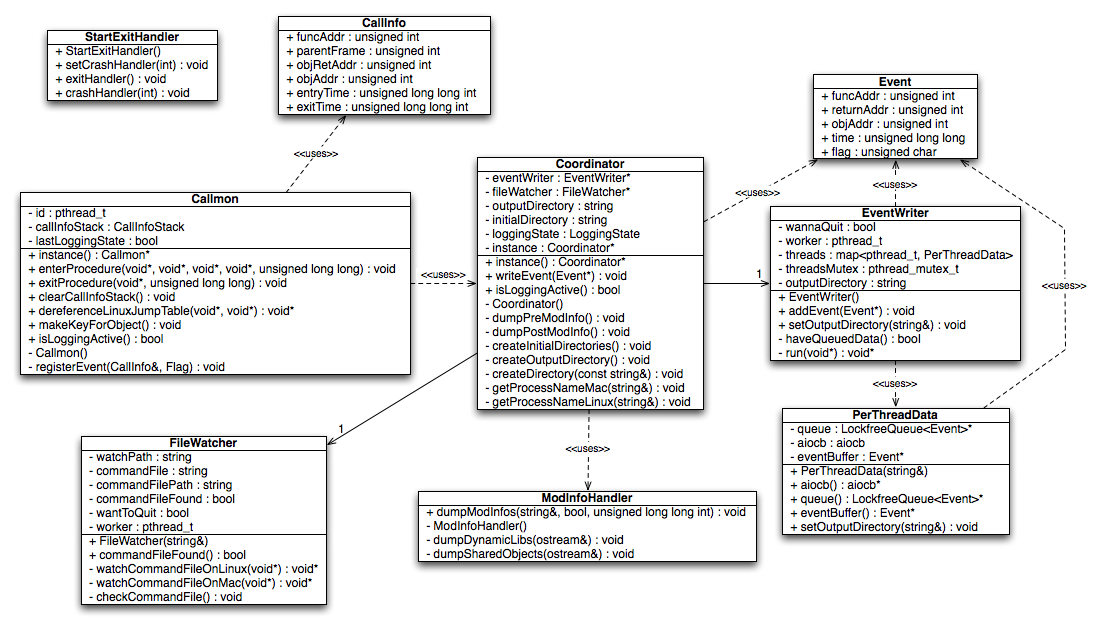
\includegraphics[width=18cm]{images/callmon_class_diagram}
\caption{Class diagram of the tracing mechanism}\label{fig:unixfe_figure1}
\end{figure}

The \emph{StartExitHandler} helps to set crash handlers for the most common signals (SIGINT, SIGILL, SIGSEGV, SIGFPE, SIGTERM, SIGABRT, SIGBUS, SIGHUP)\footnote{\url{http://en.wikipedia.org/wiki/Signal_(computing)}} and an exit handler right after startup (before main). We ensure that the constructor of the \emph{StartExitHandler} is executed before the main routine of the application with the help of a static variable. Static variables are initialized before the first call of the application main routine. The \emph{exithandler()} function deletes the \emph{Coordinator} instance. If the application crashes the crash handler gets executed which processes just a normal cleanup.\\

\emph{Callmon} provides the functionality to log function enters and exists. Every Thread of the application has its own \emph{Callmon} object. The \emph{Coordinator} is responsible to create the \emph{EventWriter} and \emph{FileWatcher}, create the directory structure for the log files and coordinates if the user wants to log. The \emph{EventWriter} runs in its own thread and receives events from all the applications threads through a lockfree queue. It uses asynchronous I/O to fill the thread specific log files. The \emph{FileWatcher} runs also in its own thread and listens on events of the file system. If a file called callmond.cmd is created or deleted we indicate this with a boolean. The \emph{ModInfoHandler} is responsible to write at the beginning or the end of the logging a list of used libraries and their start address to a modinfo file. Some classes are explained in more detail in the following sections\\

As mentioned early one of the key elements is the gcc parameter -finstrument-functions. With this option GCC inserts calls to \emph{ \_\_cyg\_profile\_func\_enter} and \emph{\_\_cyg\_profile\_func\_exit}. When an instrumented function is called, \emph{ \_\_cyg\_profile\_func\_enter} is also called, passing in the address of the function called as \emph{funcAddress} and the address from which the function was called as \emph{callSite}. When a function exits, the \emph{\_\_cyg\_profile\_func\_exit} function is called, passing the function's address as \emph{funcAddress} and the actual site from which the function exits as \emph{callSite}.\\

We implemented both functions (see callmon.cpp), which collect the following data if logging is active:
\begin{itemize}
	\item Function address
	\item Call site
	\item Frame pointer
	\item Parent frame pointer
	\item Object pointer (this pointer)
	\item Entry and exit time
\end{itemize}

In the linux case we have one special characteristic in the \emph{ \_\_cyg\_profile\_func\_enter} to resolve the function address. We have to correct the function address with the help of \todo{TODO: dereferenceLinuxJumpTable}, because the address might be wrong if the call went into a shared library.\\

Figure \ref{fig:unixfe_figure2} illustrates the whole logging process for one \emph{ \_\_cyg\_profile\_func\_enter}. \todo{explain the whole process}

\begin{figure}[ht]
\centering
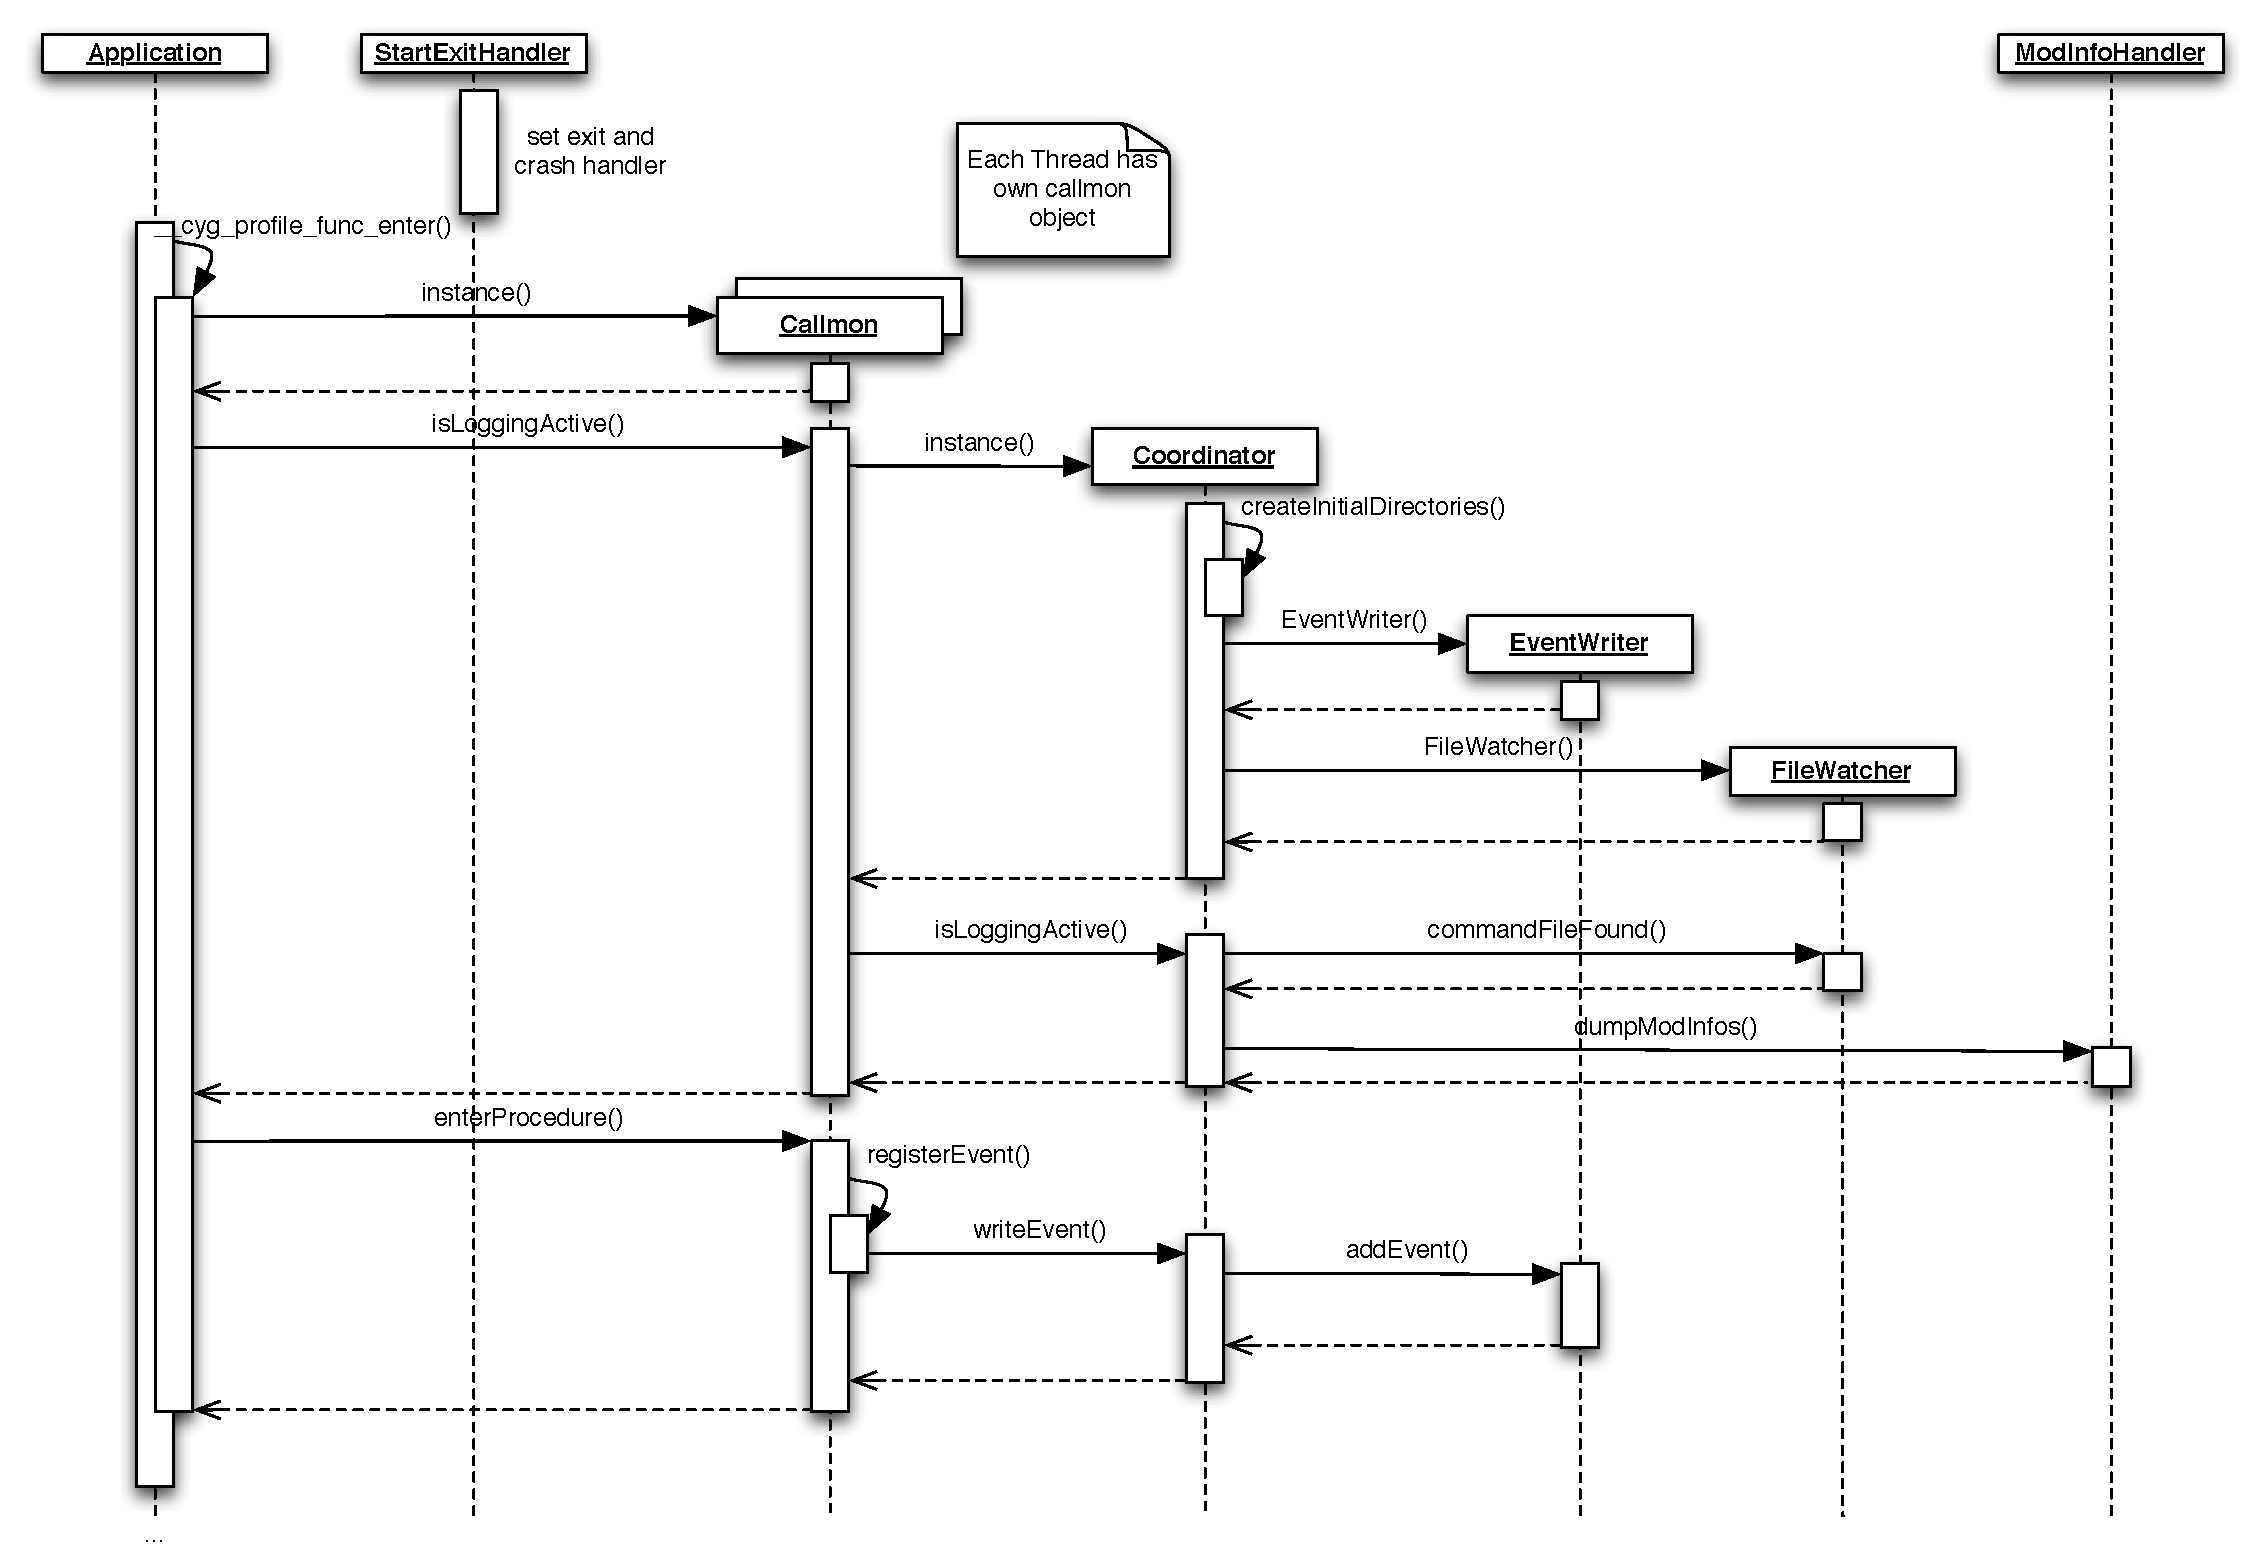
\includegraphics[width=18cm]{images/callmon_sequence_diagram}
\caption{Sequence diagram of the function enter process}\label{fig:unixfe_figure2}
\end{figure}


\begin{verbatim}
enter procedure, exit procedure
\end{verbatim}

callinfostack, shadowstack

thread local storage
Callmon singleton pro thread (lazy initialization, is the tactic of delaying the creation of an object, the calculation of a value, or some other expensive process until the first time it is needed.)

Event explain format:
function address, return address, object address, time, flag (entry or exit)

\subsubsection{Coordinator}

singleton

Coordinator - create initial directories (get proc names, linux and mac), modinfohandler, isLoggingActive, output directory

\subsubsection{Modinfo handler}
format

\subsubsection{Filesystem events}

linux filesystem watching

mac file system watching

cga toolbar

\subsubsection{Lockfree event to disk} 

\subsubsection{Asynchronous IO}

\subsection{Patch and Patchclean} 

\subsubsection{ELF patching} 

\subsubsection{MachO patching}

\subsection{Metacreator} 

\subsubsection{Line number caching} 
